\chapter{Stochasticity of the evolution}
In the previous chapters, we derived an approximated expression for the exit times using the high-dimensional
ordinary differential equations of the process.
The results obtained were only partially satisfactory, as they only partially captured the exit-time trend,
allowing us to make assertions only about the orders of magnitude of the gain obtained by overparameterizing the neural network.

In this chapter we will introduce corrections to the differential equations we have previously used,
transforming them into stochastic differential equations, with the aim of having an exact expression of exit time.
We will focus only on phase retrieval, given the simplicity of the equations it involves. 

\section{Stochastic differential equations}
There are two main problems affecting the results on the exit times of the previous chapter.
The first one is that the differential equations are valid in the limit~\(d\to+\infty\),
but then we use big, but still finite, \(d\) for comparison. 
The second problem is that Theorem~\ref{thm:process_to_ode_goldt} explicitly says that the solution of the differential equation approximates the trajectories with an accuracy that scales as \(\frac{1}{\sqrt{d}}\),
which is of the same order as the variation in the order parameters we are trying to measure.
Although we collect some statistics by simulating different trajectories,
the differential equations do not seem to be sufficient to have an accurate estimate of the exit time.

The ordinary differential equations were derived as the limit of a discrete stochastic process.
All random components were canceled by the limit procedure, leaving simply the expectation value of the random variable.
Rewriting the Equations~\eqref{eq:genericODE}, in the case \(k=p=1\) we have 
\[\begin{split}
  \dod{\left[\M{\left(t\right)}\right]_{11}}{t} &=\E_{\vec{\lf},\vec{\lf^* \sim \gauss{(0,\vec{\Omega}{(t)})}}}{\left[\mathcal{M}\right]} \\
  \dod{\left[\Q{\left(t\right)}\right]_{11}}{t} &=\E_{\vec{\lf},\vec{\lf^* \sim \gauss{(0,\vec{\Omega}{(t)})}}}{\left[\mathcal{Q}\right]},
\end{split}\]
where we have introduced the two random variables
\[\begin{split}
  \mathcal{M} \coloneqq &  \frac{\gamma}{p} \dsp_1 \lf_1^* \\
  \mathcal{Q} \coloneqq &  \frac{\gamma}{p}\left(\dsp_1 \lf_1 + \dsp_1 \lf_1\right) + \frac{\gamma^2}{p^2} \dsp_1^2
\end{split}\]
What we want to do is to include correction terms that incorporate the next order in \(d\).
Obviously, the correction cannot be deterministic since the limit is computed on a random variable;
moreover, it will have to have zero expectation value, otherwise, it would go to change order 0.
The simplest model we can imagine is given by introducing white noise that has as its intensity the standard deviation of the variables on which the expectation values are computed.
In other words, in the passage to the limit, instead of turning the random variables into expectation values,
we instead replace them with Gaussians that best approximate the random variables.
Let's put these considerations into formulas. We can start by defining the covariance matrix of \(\mathcal{M}\)
and \(\mathcal{Q}\)
\[
  \vec{\Sigma} \coloneqq 
  \begin{pmatrix}
    \Var{\left[\mathcal{M}\right]} & \Cov{\left[\mathcal{M},\mathcal{Q}\right]} \\
    \Cov{\left[\mathcal{M},\mathcal{Q}\right]} & \Var{\left[\mathcal{Q}\right]}
  \end{pmatrix},
\]
from which we can define the standard deviation vectors
\[
  \begin{pmatrix}
    \vec{\sigma}_m \\
    \vec{\sigma}_q
  \end{pmatrix}
  \coloneqq
  \sqrt{\vec{\Sigma}}.
\]
We introduce the noise as a differential vector of Wiener processes, one per equation
\[
  \dif \vec{W} \coloneqq 
  \begin{pmatrix}
    \dif W_m \\
    \dif W_q
  \end{pmatrix}
\]
where \(W_m\) and \(W_q\) are 2 independent Wiener processes.
What was previously a system of ordinary differential equations now becomes a system of stochastic differential equations.
Referring to Equations~\eqref{eq:genericODE} for notation, and eliminating subscripts since we are focusing on phase retrieval
\begin{subequations}\label{eq:unconstrainted_phase_retrivial}\begin{align}
  \dif m =& \Psi{(m,q)}\dif t + \frac{\vec{\sigma}_m{(m,q)}\cdot\dif \vec{W}}{d} \\
  \dif q =& \Phi{(m,q)}\dif t + \frac{\vec{\sigma}_q{(m,q)}\cdot\dif \vec{W}}{d} 
\end{align}\end{subequations}
Obviously, in the limit \(d\to+\infty\) we fall back to ordinary differential equations,
since the stochastic term cancels out.
These equations describe the evolution of the unconstrainted phase retrieval,
which will be the first case we are going to analyze in the next section.

One issue that needs to be addressed before continuing is the choice of the type of stochastic integration to be used for our situation.
The SDEs were obtained as a continuous limit of a discrete stochastic process so the most suitable integration is the Itô one~\cite{smith2018ito}.
There is no reason to believe that the noise is correlated with the future step of the process, 
therefore we can assume the integral of the pure noise should be a martingale.

\subsection{Initial conditions}
Before we go to simulate the stochastic process, we must choose what initial conditions to use.
Since our goal is to find a description of the learning process that is able to detect effects that escaped the differential equations,
we will look at the situation where they strayed furthest from the simulation. 
We therefore choose to initialize the phase retrieval with the \emph{symmetric intial conditions with \(\varepsilon = 0\)} (see the \ref{subsec:symmetric_init} section).
In our context we can also assume \(q_0 = 1\): this basically means choosing the vectors \(\w\) and \(\w^*\) as orthogonal
\[
  q(0) = 1, \quad m(0) = 0 \quad\text{and}\quad\rho=1.
\]

As already shown, the description with differential equations is not able to break the initial symmetry and the vectors remain orthogonal throughout the process,
changing only the norm of \(\w\).
In contrast, we expect the stochasticity introduced by the corrective term to lead to symmetry breaking and a consequent correct description of the learning process.

Finally, we choose to study the case with \(\Delta=0\). 
This choice follows from the fact that in the past chapters we have shown that the value of noise only marginally affects the first part of the process,
i.e., the part we want to study. Therefore, we choose to exclude it in order to have a less complex,
but no less descriptive, description of the process.


\section{Unconstrainted Phase retrieval}
We can now turn to test the model we introduced in the previous section.
The value of \(\Phi\) and \(\Psi\) is known from Equations~\eqref{eq:phase_retrieval},
while the matrix \(\vec{\Sigma}\) is calculated in Appendix~\ref{app:std_sde}.

\begin{figure}
  \centering
  \begin{subfigure}{0.75\textwidth}
    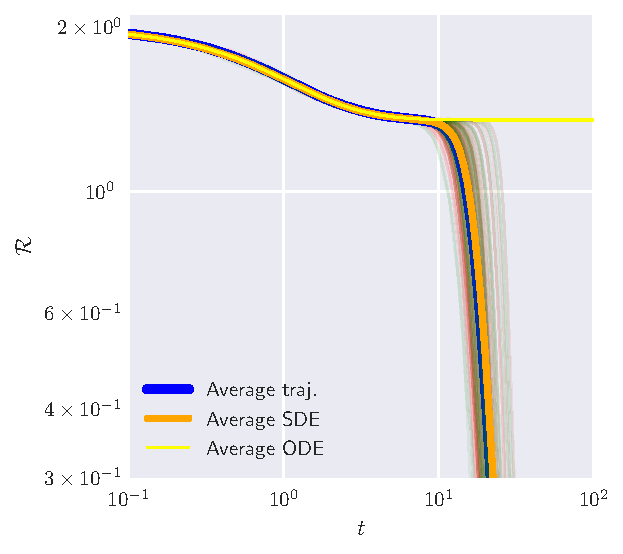
\includegraphics[width=1.\textwidth]{figures/sde/unconstrainted-sde-example.pdf}
    \caption{general trend}
  \end{subfigure}
  \begin{subfigure}{0.75\textwidth}
    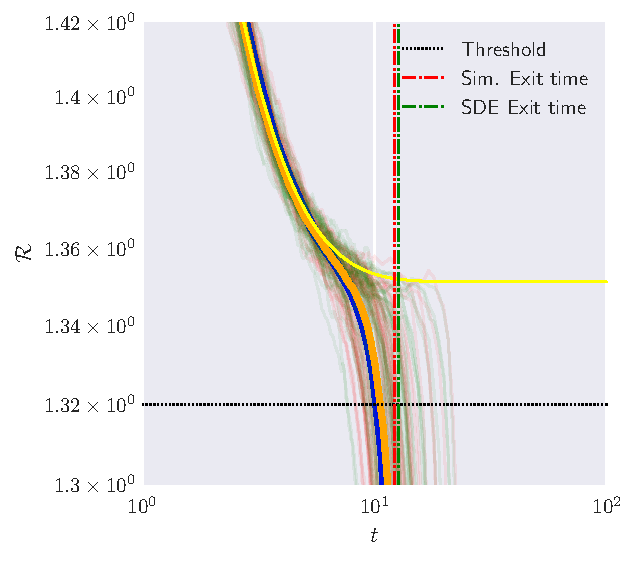
\includegraphics[width=1.\textwidth]{figures/sde/unconstrainted-sde-example-zoom.pdf}
    \caption{zoom on separation zone}
  \end{subfigure}

  \caption{
    comparison between simulation and theory with \(\gamma=\num{0.1}, \Delta=0\).\\
    The shaded red lines represent the different simulated trajectories,
    while the shaded green lines are different realizations of the solution of the stochastic process.
  }
  \label{fig:unconstrainted-sde}
\end{figure}
Figure~\ref{fig:unconstrainted-sde} shows the result of a simulation.
The first thing to observe is that, as we expected, the solution of the differential equations is not able to break the symmetry.
Conversely, the description through the stochastic process is not affected by this problem,
being able to emulate the results obtained by training the complete network.

In the figure, the individual trajectories used to evaluate both the simulation and the process obtained from the SDEs are also shown:
we can see how the distributions seem to overlap, a symptom of the fact that the stochastic process has the same distribution as the complete network.
As evidence for this claim, we calculated two different statistics to compare:
the average trajectory and the time to exit a threshold.
Both coincide within the experimental error, which, however, cannot be eliminated having used a finite number of samples (56 for each).

The result is in agreement with what was recently reported in a paper by G. Ben Arous et al.\cite{arous2022high}.
In the paper, it is shown that in the high-dimensional limit of an optimization performed with SGD,
the dynamics of summary statistics (order parameters) can be described by Brownian motion.
We have explicitly written Brownian motion for the phase retrieval, and numerical simulations confirm that the dynamic is just that.

As we had already found in the study of ordinary differential equations,
the unconstrained phase retrieval does not allow us to derive a formula for exit time since it is not possible to make expansions and solve the process analytically.
We will therefore proceed to constrain the dynamics on the sphere, exactly as done in the last chapter.

\section{Spherical Phase retrieval}
In this Section, we extend the treatment with stochastic processes to constrained dynamics on the sphere.
We note that constrained dynamics is not a case included in the results of Ben Arous \cite{arous2022high}
since the imposition of the constraint is not writable as a gradient of a function.

We first show that trying to derive the stochastic correction directly by estimating the variance of the drift term leads to incorrect results. 
We will then proceed with a derivation using the Itô Calculus, which although not completely formal,
still leads to the correct description of the dynamics

\subsection{Naive derivation}
The first attempt we did for computing the variance of the process consists of writing 
the differential equation of phase retrieval (Equation~\eqref{eq:spherical-phaseretrivial}) an expected value 
\[\begin{split}
  \dod{m}{t} =& \Psi -\frac{m(t)}{2}\Phi = \E_{\vec{\lf},\vec{\lf^* \sim \gauss{(0,\vec{\Omega}{(t)})}}}{\left[\mathcal{M}\right]} - \frac{m(t)}{2}\E_{\vec{\lf},\vec{\lf^* \sim \gauss{(0,\vec{\Omega}{(t)})}}}{\left[\mathcal{Q}\right]} \\
             =& \E_{\vec{\lf},\vec{\lf^* \sim \gauss{(0,\vec{\Omega}{(t)})}}}{\left[\mathcal{M}-\frac{m(t)}{2}\mathcal{Q}\right]}
             \coloneqq \E_{\vec{\lf},\vec{\lf^* \sim \gauss{(0,\vec{\Omega}{(t)})}}}{\left[\mathcal{M}_S\left({m(t)}\right)\right]}
\end{split},\]
where we have introduced the random variable \(\mathcal{M}_s\) as a linear combination of the other two.

We can now think to write the process using the variance of \(\mathcal{M}_S\) as noise term.
\[
  \dif m = -\frac{m{(t)}}{2}\left[8\gamma(1-6\gamma)(m^2{(t)}-1)+4\gamma^2\Delta\right] \dif t
           + \frac{\sqrt{\Var{\left[\mathcal{M}_S\right]}}}{d}\dif W.
\]
The drift term comes from Equation~\eqref{eq:spherical-phaseretrivial}, while the explicit form of \(\Var{\left[\mathcal{M}_S\right]}\)
can be found in Appendix~\ref{app:std_sde}.

We tried to simulate this stochastic process; results are in Figure~\ref{fig:naive_sde_pr}.
\begin{figure}
  \begin{center}
    \includegraphics[width=0.6\textwidth]{example-image-duck}
  \end{center}
  \caption{}
  \label{fig:naive_sde_pr}
\end{figure}
It's not correct because... TODO: Comment the Figure!

\subsection{Itô Calculus}

The idea we develop in this section is to write the constrained update rule for \(m\) as a function of the unconstrained differentials \(\dif m, \dif q\),
derived in Equation~\eqref{eq:unconstrainted_phase_retrivial}.
At that point using the Itô Calculus we will derive the stochastic process describing the learning bound to the sphere.
To avoid ambiguity in the computation, we denote by \(\dif m_S\) the constrained differential, while \(\dif m\) is the unconstrainted one.

Starting from the unconstrainted update rule for the weights (Equation~\eqref{eq:update_rule_weights}),
we can find an expression for the two unconstrainted differentials
\[\begin{split}
  \dif q &= \frac{-2\gamma \w\cdot\nabla{\loss} + \gamma^2\left\|\nabla{\loss}\right\|^2}{d} \\
  \dif m &= \frac{-\gamma \w^*\cdot\nabla\loss}{d}.
\end{split}\]
Since we are forcing the weight on the sphere, the update rule that has to be used is
\[
  \w^\text{update} =\frac{\w - \gamma \nabla{\loss}}{\left\|\w - \gamma \nabla{\loss}\right\|}\sqrt{d};
\]
multiplying both sides by \(\w^*\) and subtracting \(m\) we get
\[
  \dif m_S = \frac{m +\dif m}{\left\|\w - \gamma \nabla{\loss}\right\|}\sqrt{d} - m.
\]
Let's estimate the normalization factor
\[
  \begin{split}
  \left\|\w - \gamma \nabla{\loss}\right\| =& \sqrt{(\w - \gamma \nabla{\loss})^2}
                                           =  \sqrt{\w^2 - 2\w\cdot\gamma \nabla{\loss}+\gamma^2\left\|\nabla{\loss}\right\|^2} \\
                                           =& \sqrt{d}\sqrt{\frac{\w^2}{d} + \frac{- 2\w\cdot\gamma \nabla{\loss}+\gamma^2\left\|\nabla{\loss}\right\|^2}{d}}
                                           = \sqrt{d}\sqrt{q +\dif q} \\
                                           =& \sqrt{d}\sqrt{1 +\dif q},
  \end{split}
\]
where in the last step we used the constraint \(q=1\). We can now plug it back in \(\dif m_S\)
\[
  \dif m_S = \frac{m +\dif m}{\sqrt{1 +\dif q}} - m,
\]
and expanding up to leading orders we get
\[\begin{split}
  \dif m_S =& (m +\dif m)(1 +\dif q)^{-\frac12} - m = (m +\dif m)\left(1 -\frac12\dif q + \frac38\dif q^2\right)-m \\
           =& \dif m - \frac{m}{2}\dif q -\frac12 \dif m \dif q + \frac38 m \dif q^2
\end{split}\]
We can now use the Itô Lemma on differentials Equations~\eqref{eq:unconstrainted_phase_retrivial},
obtaining 
\[
  \dif m^2 =    \frac{\vec{\sigma}_m^2}{d^2}\dif t, \quad
  \dif q^2 =    \frac{\vec{\sigma}_q^2}{d^2}\dif t, \quad\text{and}\quad
  \dif m \dif q = \frac{\vec{\sigma}_m  }{d^2}\cdot \vec{\sigma}_q \dif t.
\]
Using them combined with Equations~\eqref{eq:unconstrainted_phase_retrivial} we can finally write
the explicit Brownian motion for the constrained dynamic
\begin{equation} \label{eq:constrained_brownian_motion}
  \dif m_S = \left(\Psi - \frac{m_S}{2}\Phi\right)\dif t
            + \frac{1}{d}\left(\vec{\sigma}_m-\frac{m_S}{2}\vec{\sigma}_q\right)\cdot \dif \vec{W}
            + \frac{1}{d^2}\left(-\frac12\vec{\sigma}_m \cdot \vec{\sigma}_q +\frac38 m_S \vec{\sigma}^2_q\right)\dif t.
\end{equation}
Of course, all functions should be evaluated at \(m=m_S, q=1\).
We can see that there is an extra drift term in addition to the one also found in the ODEs.
Although the correction the extra drift introduces is at the second order,
nevertheless we include it in our analysis since the effect it introduces is deterministic.

Equation~\eqref{eq:constrained_brownian_motion} describes the full spherical process,
but it's still too complicated to be used for deriving an exit time formula.
We have to find an approximation for the first phase of the process. As we did 
for the ordinary differential equations, since we start at \(m_S=0\), we can keep on linear terms in the drift;
moreover, we can assume the noise in the starting plateau to be constant, using the values reported in Appendix~\ref{app:std_sde}.
The process takes the form 
\[\begin{split}
  \dif m_S = \mu m_S \dif t + \sigma \dif W \quad \text{with}\\
  %
  \mu = 4\gamma(1-6\gamma)-2\gamma^2\Delta+\frac38 \vec{\sigma}^2_q\quad\text{and}\quad
  \sigma = \frac{\vec{\sigma}_m}{d}
\end{split}\]
The same considerations on learning rate bounds we discussed in Section~\ref{sec:spherical_phase_retrivial} apply also here.
The approximated evolution of \(m_S\) is a \emph{expansive Ornstein–Uhlenbeck} process, since \(\mu>0\).
We have already shown that in the phase retrieval there is a direct map between \(m\) and the theoretical risk;
we can deal just with the order parameter \(m\) for the exit time. 
Given an expansive OU-process staring at \(m_S=0\), the mean first exit time from the interval \((-r,r)\) is given~by~\cite{zeng2020mean}
\[
  t^{(\text{pr})}_e = \frac{r^2}{\sigma^2} \prescript{}{2}F_2{
    \left(1,1; 3/2,2; 
  -\frac{\mu}{\sigma^2}r^2\right)}
\]
where \(\prescript{}{2}F_2\) is a generalized hypergeometric function;
see Appendix~\ref{app:math_tools} for reference.
The formula does not have a closed form like the one derived earlier,
but still, it could be used for the asymptotic study of exit time.
Figures~\ref{fig:comparison_te_ode_sde} shows different perspectives of comparisons 
between the ODE formula and the SDE one. Although the stochastic process does not incorporate
any dependence on \(d\) in the initial conditions, it is still able to capture the same global trend for exit time.
This supports the work we did to calculate the gain in the last chapter,
showing that even by correcting the process description, however, 
the global result does not change considerably, and the corrections are not dominant in the final formula.
\begin{figure}
  \centering
  \begin{subfigure}{0.495\textwidth}
    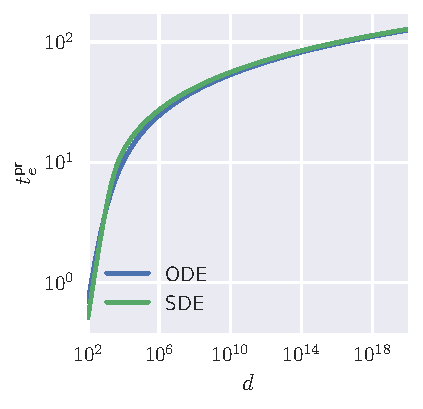
\includegraphics[width=1.\textwidth]{figures/sde/ode_vs_sde_r0.05.pdf}
    \caption{\(r=\num{5e-2}\) global view}
  \end{subfigure}
  \begin{subfigure}{0.495\textwidth}
    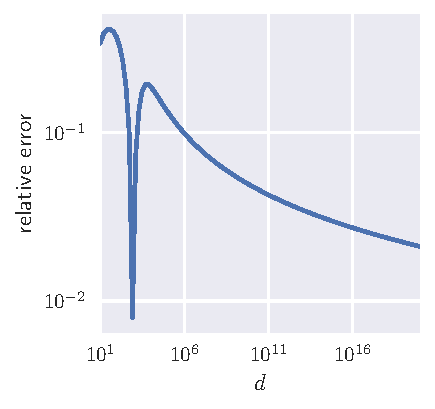
\includegraphics[width=1.\textwidth]{figures/sde/ode_vs_sde_relative_error.pdf}
    \caption{\(r=\num{5e-2}\) relative error}
  \end{subfigure}
  \begin{subfigure}{0.495\textwidth}
    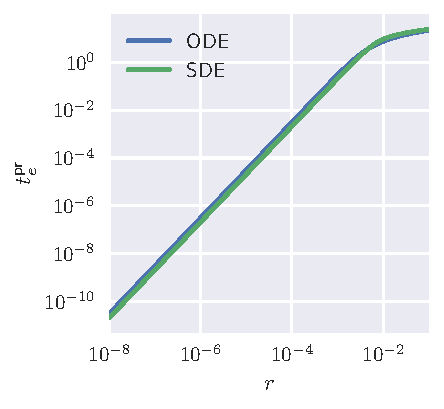
\includegraphics[width=1.\textwidth]{figures/sde/ode_vs_sde_d1e5.pdf}
    \caption{\(d=\num{1e5}\)}
  \end{subfigure}
  \begin{subfigure}{0.495\textwidth}
    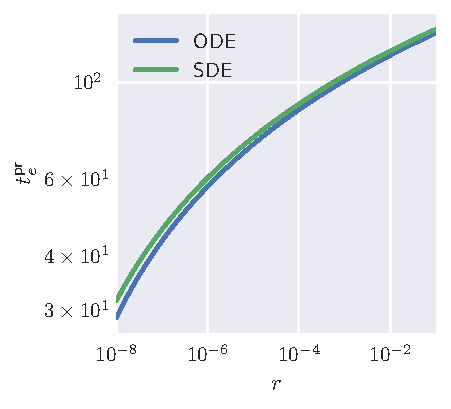
\includegraphics[width=1.\textwidth]{figures/sde/ode_vs_sde_d1e20.pdf}
    \caption{\(d=\num{1e20}\)}
  \end{subfigure}
  \caption{
    comparison between the theoretical exit time obtained with the ODE and the one obtained from SDE.
    Parameters: \(\gamma=\num{0.1},\Delta=0\).
  }
  \label{fig:comparison_te_ode_sde}
\end{figure}

Let's conclude by presenting the numerical simulation to test our new exit-time formula.
\begin{figure}
  \centering
  \begin{subfigure}{0.495\textwidth}
    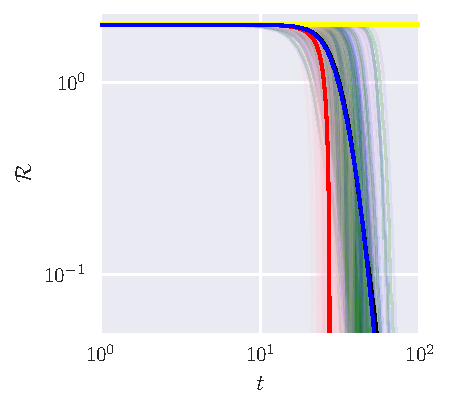
\includegraphics[width=1.\textwidth]{figures/sde/spr_final.pdf}
    \caption{global view}
  \end{subfigure}
  \begin{subfigure}{0.9\textwidth}
    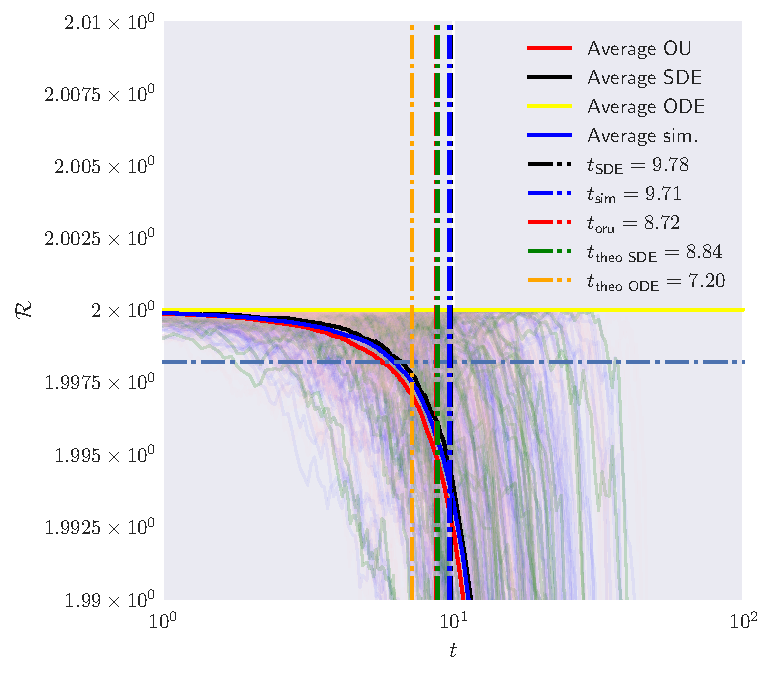
\includegraphics[width=1.\textwidth]{figures/sde/spr_final_zoom.pdf}
    \caption{zoom}
  \end{subfigure}
  \caption{
    comparison between different exit time measurements and estimations.
    Parameters: \(d=10000, \gamma=\num{0.1},\Delta=0\).
  }
  \label{fig:spr_final}
\end{figure}
Figure~\ref{fig:spr_final} shows the results. The stochastic process described by Equation~\eqref{eq:unconstrainted_phase_retrivial}
is able to catch the dynamic of the real neural network quite well, while the ODEs get stuck in the symmetry.
The difference between measured exit time from the simulation and from the stochastic process is below the numerical error.
This confirms once again that the path we followed for the correction term is right.
The approximated stochastic process (Ornstein-Uhlenbeck) is not perfectly matching the complete one.
\(t_\text{oru}\) is not compatible with \(t_SDE\), but still is a good approximation.
This difference is caused by the approximations we took to arrive at an analytically tractable process;
better results could be obtained by decreasing the threshold \(r\). 
As expected, the theoretical formula is compatible with the time measured on the approximated process,
but it suffers from the same problems mentioned above when it comes to measuring the time of the complete process.
Finally, we note that the formula obtained by manipulating the SDEs is considerably more accurate than that obtained from the ODEs. 

In conclusion, the use of stochastic processes allowed us to arrive at a better formula than the one found in the previous chapter. This is the right direction for future investigations.